% This example An LaTeX document showing how to use the l3proj class to
% write your report. Use pdflatex and bibtex to process the file, creating 
% a PDF file as output (there is no need to use dvips when using pdflatex).

% Modified 

\documentclass{l3proj}
\usepackage{hyperref}

\begin{document}

\title{ ScriptSpeare}

\author{Ivan Delev \\
        Bita Fardroo \\
        Muhammad Fahd Asif \\
        Sofia Simola \\
        Erlend Frayling\\
        Kristupas Liubinas \\}

\date{08/04/2019}

\maketitle

\begin{abstract}

The report talks about the 3rd year project of the CSP2 team consisting of six joint honours student. The project focuses on designing a web application for the client Scriptate, which would allow interaction with Shakespeare plays. The report will be discussing the nature of the product and the processes to develop the final version which was launched on www.scriptspeare.co.uk. Overall the report explores the challenging and enriching steps that lead towards a successful goal. 

% Project description: this project focused on creating media player controls for an interactive script player system, focused on usability, easy user interaction, along with the flexibility of making the media player personalised for each individual user.

\end{abstract}

%% Comment out this line if you do not wish to give consent for your
%% work to be distributed in electronic format.
\educationalconsent

\newpage

%==============================================================================
\section{Introduction}

This paper presents a case study of CSP2, a group of six undergraduate joint-honours Computing Science students at the University of Glasgow, and their experiences developing a software project for a real-life customer, as a professional software development team. The project was undertaken as part of the students’ 3rd year curriculum on the course ‘Team Project 3’, ran in conjunction with the ‘Professional Software Development’ course.  The purpose of the case study is to present the group’s software development process, analyse their adopted work practices and reflect on the lessons learned during the project. The report will explore the case study, the workflow of the team, the development processes and the choice of technologies. Key challenges of the project will be discussed with a final reflection and conclusion stated.


% Software engineering 

% This paper presents a case study of... 



% %% Final paragraph.
% The rest of the case study is structured as follows.  Section
% \ref{sec:background} presents the background of the case study
% discussed, describing the customer and project context, aims and
% objectives and project state at the time of writing.  Sections
% \ref{sec:alice} through Section \ref{sec:managing} discuss issues that
% arose during the project...

%==============================================================================
\section{Case Study Background}

% Include details of 

% \begin{itemize}
% \item The customer organisation and background.
% \item The rationale and initial objectives for the project- these points are discussed in section 3, please do go through the aims and initial planning.
% \item The final software was delivered for the customer.
% \end{itemize}


\subsection{Project Customer}

The team worked on a project presented by a Glasgow based start-up company called Scriptate. Ran by the co-founders Andrew Maguire and Christopher Westerduin, the company provides transcription and subtitling service to organisations and individuals. According to the founders, the service delivers “interactive transcripts which viewers use to instantly find a moment within audio-visual content, combining automation such as speech recognition with personalised human curators”  \cite{edgeapp}. Mr Maguire and Mr Westerduin were the main company representatives with whom the students interacted throughout the development of the proposed project.

\subsection{Customer's Objectives}

Through collaboration with the University of Glasgow students, Scriptate aimed to develop a program that would enable people to interactively explore plays written by William Shakespeare. The program would act as a centralised platform for Shakespeare’s scripts, collecting a variety of adaptations (films, theatre recordings, audio-books) around an interactive transcript of each play. Combining the best features of similar existing products such as The Tempest app \cite{heuristics}, Shakespeare’s Sonnets app \cite{ssonnets}, ShakespeareWords.com \cite{swords} and others, the company recognises such applications as an innovative way to offer their transcription service to new markets (schools, actors, etc). Specifically, the customer expected the CSP2 team to develop a media control interface which would act as the centre for user interaction with Shakespeare’s script and corresponding audio-visual adaptation.

\subsection{Achieved Product}

In collaboration with a group of single-honours students responsible for the back-end development, CSP2 developed a web application based on the Django framework. Focusing mostly on the UI aspects of the website and working from scratch (that is, without utilizing any software already developed and/or used by the company. This was done per customer’s request) the team delivered all core concept features outlined in the initial project proposal. Those were a) enabling users to jump to specific points in the accompanying media through the text; b) seamlessly switching to the same line between different adaptations; c) looping specific sections of the text to memorize lines. In addition, the students created a user interface to facilitate the aforementioned functionality and delivered an additional feature of tracking and highlighting the currently played line in the media file. The final product, named ScriptSpeare, was deployed online and is accessible at https://scriptspeare.co.uk/.



%==============================================================================
\iffalse

\section{Aims, Initial Planning and Requirements}

\subsection{Initial Planning}

To gather the user requirements, the front-end team met to discuss them. After dividing the tasks among themselves, the team started to work on their assigned tasks, while coherently following the lecture slides (from the PSD module).

Once the user stories and user personas were prepared, the team met with the client to discuss them (along with the wireframes). Following the meeting, the suggestions made by the client were considered, and the team started to work changes into them.

The client came with a list of features and user requirements, prior to the first customer day. After several meetings, the team successfully negotiated with the client.The user requirement documentation was finalised prior to the customer day where it was presented to the client. The development of the web application was started after this meeting.

\subsection{Requirements}

\subsubsection{1st and 2nd Customer Days}

Requirements gathered up to and including the first customer day were as follows:  

\begin{itemize}
\item Develop a webpage for the Media player (similar to that in the wireframes);
\item Media player must have a customisable play bar, with several options (similar to those in the wireframes);
\item Interactive Script - once a dialogue is selected, interactive script should allow the user to jump to the same (clicked) dialogue in the video. 
\end{itemize} 

In short, the front-end team promised to develop a web page, which would be containing an intuitive video media player. Furthermore, a script would be shown on the right-hand side of the video player. The user will be able to interact with the script, hence allowing them to use some functionalities such as jumping to a specific dialogue in the video and looping through the dialogues.   

A meeting was scheduled between both teams where it was discussed that the front-end team would work on the media player and pull the video and audio from the database, which was going to be setup by the back-end. 

As the client was enthusiastic about their product, they would at times bring new requirements for the team in those meetings. As a result, the client was requested to message the relevant team members (communicators) before coming to our meetings, so that operations would run smoothly.

Targets achieved up to and including the second customer day were as follows:

 \begin{itemize}
\item Completed the initial designs including wireframes and dummy buttons;  \cite{wireframes}
\item Gathered epic user stories and personas to enhance the understanding of the requirements;
\item A basic Prototype was assembled (with promised features);
\item Teams developed a thorough understanding of web technologies.
 \end{itemize}

Negotiated requirements gathered up to and including the second customer day are as follows:
 \begin{itemize}
\item  Created a home page, with the option of choosing categories, like comedy/tragedy; then allowing the users to pick a play from each category of their choice;
\item  Integration of the initial media player (web page) with Django;
\item  Make the script more interactive-  Change from a “Select” loop function to a “Drag” loop function etc.;
 \end{itemize}

\subsubsection{3rd Customer Day}

For this iteration, the team came to realise about this parser in the middle of the iteration, when some members from the front-end team met with others from the back-end team. 
All in all, the team was successfully able to achieve these targets:
\begin{itemize}
\item Desired “Home” page was developed;
\item  Implementation of the buttons to the media play bar, while making the script more interactive;
\item Learnt about branches (on Gitlab) and Django;
\end{itemize}

Some of the requirements gathered before (and including) the third customer day were as follows:
\begin{itemize}
    \item Responsive design for website/web app;
\item Discussed the implementation of Parser and how it could be developed and used;
\end{itemize}

\subsubsection{4th Customer Day}
A meeting was scheduled to discuss the IP of the project, and it was agreed that the license was going to be an open source. 
Overall, some notable targets achieved up to and including the fourth customer day were as follows:
\begin{itemize}
    \item  Parser development and integration had begun;
\item The integration from the back-end’s database had begun, as the mp4 files from the back-end’s database were getting pulled by the media player while functioning properly;
\item Started testing the integration (with the back-end’s database);
\item Multi-tier drop-down menu construction had begun;
\end{itemize}

Some of the revised user requirements gathered upto and including fourth customer day were as follows:
\begin{itemize}
    \item Deployment of website on the client’s domain;
\item  Integration process to be continued whenever the singles database is ready;
\item Finalising the media player by tweaking the home and the media player page, so that the application becomes more visually pleasing;
\item Fix the bugs within the website after the deployment of the web application;
\item Finishing up the product as desired by the client.
\end{itemize}

\subsubsection{Final Customer Day}
Straight after the fourth customer day, a license search was carried out by one of the team members. Necessary actions were taken by both the teams to launch the website successfully on the client’s domain. After the launch, the website was debugged, so that the website worked more efficiently and looked more professional. 
The final targets achieved up to and including the final customer day were as follows:
\begin{itemize}
\item The team decided to use APACHE 2.0, as an open source License for the application;
\item The web application was deployed on the client’s domain;
\item The multi-tier drop-down menu with search features was installed on the application;
\item  Highlighting the current line played by the media player;
\item Numbering the lines through-out the entirety of the script;
\item  Moving between adaptations while keeping the current line;
\item  Appropriate URL displayed on the browser for the deployed website;
\item Collaboration with two teams;
\item  Functioning Media Player with Interactive Script;
\item Debugging the website, like fixing the radio buttons, displaying the list of plays etc.;
\item Successful implementation of all agreed features, along with the deployment of the latest version of the application via AWS (by the back-end team). 
\end{itemize}

The requirements agreed by the front-end team through-out the entirety of the project were met. The front-end team was able to develop a media player which fulfilled the complete user requirements and satisfied the client. 
\fi

%==============================================================================
\section{Workflow processes}
\label{design}

This section will give an overview of the workflow, team roles and nature of collaboration.  It will explore how the team structured their workflow during a sprint and the collaboration with another team and show the learning curve on  communication and the challenge the project reflected due to its shared attribute.

\subsection{Team Roles}
During the iterations, the structure of the team and the specific roles kept adapting to optimize meeting the requirements of the project. Initially  fixed roles were given out, like toolsmith, librarian, main coder, and designer. \cite{mythical} However, it was quickly realised that this was restricting the team to specific tasks and changed to a dynamic approach where issues would be created at the start of each iteration and the team could decide themselves what they felt most confident on working with. 

One main change made early on was appointing a product owner. This was necessary in order to meet the demand for communication from the client’s side but also ensure the efficient workflow of the whole team.

\subsection{Planning of Iterations} 
Ideally, sprints would start with a customer meeting which would give the team the opportunity to discuss requirements for the next milestone or iteration. After the customer meeting, the team would have a planning session with the use of agile processes such as planning poker to estimate the time and resources needed for each task. The team leader would then transform those requirements into issues and the team would decide among themselves who would be doing what.  Meetings were held weekly on Wednesdays in the lab in order to discuss progress and challenges faced and to solve some issues together. At the end of each sprint, the team would do a retrospective to improve, and learn from, what has been achieved so far. Reflectively this worked out well, some challenges faced were that the team would try to accommodate new or changed requirements from the client during sprints which will be discussed under challenges. 


\subsection{Collaboration with the Singles Team}
\label{subsec:collaboration}
The customer did not require two different versions of the same product, therefore the teams were asked to collaborate and work on the same project. This made the nature of the project more complicated, since instead of organising one team and determining its workflow, the teams  were to organise within their teams while still maintaining autonomy in workflow processes.

Based on preferences, it was decided that the singe honours team would work on the back-end part of the project, while the joint honours team would work on the front-end. Accordingly, this approach made the CSP2 team dependant on the back-end team. Hence, as the other team obviously required time to set up and work on their requirements, a lot of the inter-dependencies were finished or handed over to CSP2 at a late stage of the project, such as annotations in \ref{subsec:annotations}. This caused several issues for them, especially at the end of the project. Furthermore, problems started to incur due to the delays in hand overs; this was time expensive, as a proper protocol was to be followed in order to resolve the issue. 

Initially, the communication was inadequate; on some occasions both teams were exposed to miscommunication from either each other or the client. Eventually the communication channel did mature, as teams became more accustomed to each other. More face-to-face meetings between the members of the two teams were organized to discuss specific technical problems. This decreased the amount of miscommunications and the time spent on those.  Initial setups and agreements on technologies were made in a meeting which was a professional step instead of starting off without communication. Moreover, at the later stages of the project, the deployment of the website was discussed with both teams. 

Overall CSP2 kept the back-end team and the client updated with the changes in the user requirements and bugs. The launch of website demonstrates a successful collaboration. While there were challenges in this kind of a collaborative project, the students have learned some key aspects on working with two autonomous teams. The team thinks some miscommunication could have been prevented by working closer with the other team from the beginning. CSP2 ended up assigning a person to communicate to the other team, which helped, however they lacked to see who was in charge of the singles team. Therefore setting up initial agreements on who and how to communicate and enforcing it would be beneficial.



%==============================================================================

\section{Use of software development processes}
This section will give an overview of the key features that have been used in the development process and outline a reflection of how effective they have been.

\subsection{Branching}
The team coach suggested the use of branching in a workshop since not all of the team was familiar with that. Instead of working on master and having merge conflicts,  the decision was made to create branches for each new feature that had to be worked on. During the development process, the naming of branches became more effective and the team learned the advantages behind branching even with initial doubts. Branching became challenging once they were to be merged back to master, which is discussed under Merge Request.

\subsection{Merge requests and code review}
The team initially disregarded merge requests with the thought that it would be faster if the initial developer checked everything themselves. However, problems were encountered with this approach, when merging back put the master at risk of breaking. Hence, at the 3rd retrospective, the decision was made to make merge request mandatory. After some testing for the optimal way of who to assign merge requests to, the team ended up using messages in order to identify who is currently free to review a merge request and would assign it to that person.

This development process saved us time in debugging as well as providing a broader overall code understanding for each member.  Due to unfamiliarity with merge requests unfortunately the opportunity to use commenting on GitLab, about the progress and discussion of the individual issues, was mostly missed. Instead the team had these conversations on other communication channels. For the future, it would be essential to comment on what, why and how a merge request or conflict has been resolved. 

\subsection{Pair programming}
From the beginning, the team decided to do pair programming in order to reduce mistakes and increase the learning process. Instead of assigning fixed teams a dynamic approach was taken where team members were paired together once they chose the area they wanted to work on for that iteration. It was found that overall, a good job was done in keeping pair programming as a continuous process. However, in more busy times this ended up being more difficult as time issues were pressing and it seemed less relevant to continue this process. Similarly over the holiday break periods it proved hard to continue this approach. Nevertheless, the key advantage of pair programming became evident in the way that the live observer is a great asset to the coder which reduces debugging and frustration a lot and ultimately saves time and improves code quality.

\subsection{Retrospectives }
Retrospectives were done after each iteration and improved in content, structure, and quality the more complex our requirements and goals became and the longer the team worked together. Retrospectives were the most effective tool used in order to improve the working flow and reflectively is a great agile asset for the future.  

What was learned as a team was that each member can learn from others' experiences but found it hard to communicate these to a six-person team. They quickly figured out that problem-solving and subsequently delivering more value to the client requires change in the way of working. It was found that the best way to achieve this was to have retrospective meetings after each sprint. The team would check what had been implemented from the last retrospective and evaluate that, as well as conducting a situational evaluation of the new iteration, and document what has been going well/badly and what should we continued/started/stopped. They also tried the sailboat approach but found a table more structured for our team.

\subsection{Planning Poker}
Planning poker was introduced as a suggestion of the team coach in order to have a better overview of time estimation on requirements. Overall it improved awareness of how to take on new requirements from the client by always evaluating the time a task would take as this is a key challenge. The team quickly learned the thinking process and were also able to use it in order to allocate tasks with different difficulties to different people. However, it was also noticed that Planning Poker was very time consuming and the team only had limited time together. They decided to keep the key takeaways of planning poker, taking into account the time and difficulty of a task before assigning it to someone or taking it as an extra requirement.

Reflectively it is a good agile tool which was useful to structure workloads better and for the future can be used throughout the project by, for example, setting up a platform online where teammates can input everything remotely instead of needing a whole meeting on it.  


\section{Use of Technologies }
\label{development}
This section will discuss the main technologies used and the decisions behind them as well as reflection on some technical processes.

\subsection{Design of the Media Player and the States}

The project required different actions to happen when the script would be clicked, each of those actions affecting the video on the screen. At the beginning of the second iteration a UML class diagram (figure \ref{fig:uml}) was created for these components to make sure they would not become any more coupled than necessary.
\begin{figure}
\begin{center}
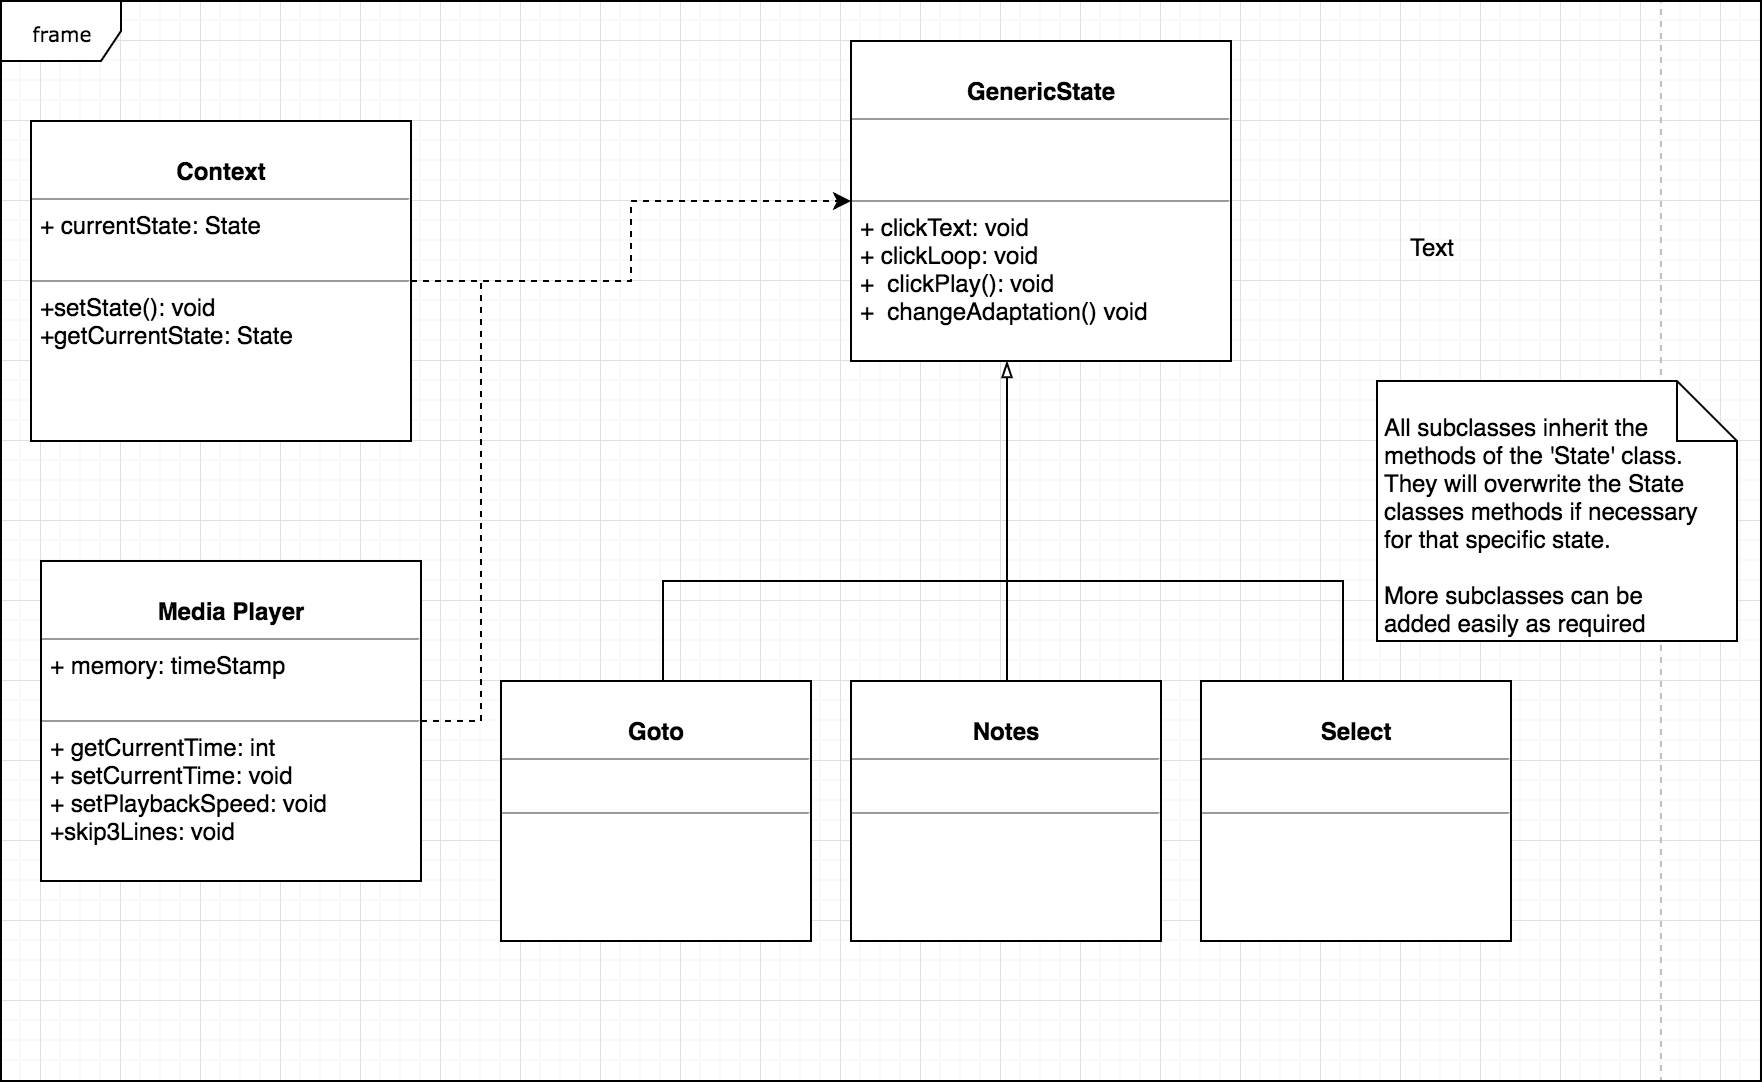
\includegraphics[width=9cm]{figures/uml_diagram}
\end{center}
\caption{The initial UML diagram for the media player and the states}
\label{fig:uml}
\end{figure}
In the actual process of implementing these using Javascript, some changes did happen. The GenericState (eventually just named ‘State’) did not contain more than a click function. Media player, on the other hand, gained more functions which were not remembered in the UML creation, such as play and pause. Despite the changes, the UML gave a good structure for the Javascript code. The process could have been improved by updating the UML more rigorously as new features came along.


\subsection{Moving to Django}
In the first semester, the web page was created solely using HTML, Javascript and CSS. This enabled quick proof-of-concept implementation and experimentation without having to learn a framework.

Around the end of the year it came time to start integrating with the back end team. For that purpose, the team decided to start migrating the webpage to the Django framework. It was not clear at that point whether users had to be created or whether the front end would need its own database, and Django provided support for both. Additionally, its templates seemed useful. Other frameworks, such as Angular, were discussed, but it was decided that learning them would take too much time.  

Working with Django was not without its hiccups - most of the team had some experience with Django, but no one was an expert. Eventually one member of the team became responsible of most Django-framework related tasks. This freed the rest of the team from having to learn the fine details of Django, but also meant that the member responsible became the first point of contact of many requests, perhaps too many, creating a harmful bottleneck for the development. Having a pair of people responsible instead of an individual would have been better.


\subsection{API Calls to the Back End}
In the fourth iteration, the back end database was finished enough to delete the hard-coded videos and start calling the videos from the AWS. This itself was quite a straightforward process.

What turned out being more difficult was removing the hard-coded drop-down menu and populating it using API calls. Initially, the Django database was used to contain all the adaptations in the web page, but this started creating conflicts when the database in AWS was updated faster than the one in Django. Therefore the database was replaced with a call to the API.

It would also have been possible not to hard-code which plays existed, but it was decided that those would change far less frequently, and could hence be hard coded on the client side.  This meant that the back end team did not have to make an API call for that and the front end team did not have to alter the existing code. If the production were to prefer long predicted lifetime of the code instead of fast production, removing this hard-coding would be necessary.


\subsection{Parser}
The customers had a number of transcript files for each adaptation. These files needed first to be turned into JSON or XML by the back-end and then into HTML by the front end. From the very beginning it was clear that neither the format of the input or the output of the front-end parser was perfectly understood. At the start the project suffered, because the communication channel between the teams was not well-established, as discussed in the section \ref{subsec:collaboration}.

The parser output from the back-end was initially to be XML, however the back-end team changed the output to JSON for convenience at their end - there was a tool, Gentle \cite{gentle}, that helped their process. Luckily, their web page contained code that could be used as a basis for the JSON parser.  From there the teams started a back-and-forth process of trying to find what all information the JSON needed. 

Simultaneously, the customer wanted to launch a prototype of the web page, and the back-end parser was the only thing holding the process back. The customer suggested using unmodified Gentle output of their script files, which they had manually created a while back. This resolved the issue of needing to have the back end parser working, although it meant some more work for the front end. Yet, it turned out that turning the annotations in the script files into HTML was easier than working with the HTML transcript provided by the back end parser. What started out as a hacky solution to the customer needing the functionality fast, turned out to be a far easier implementation approach.

The process could have used better quality assurance, section  \ref{subsec:testing} talks about this and other problems with testing. Overall, the parser should have been prioritised more than it was by both teams. As a very central component, it should have had more people working on it earlier on, and had more quality assurance.


\subsection{Annotations}
\label{subsec:annotations}
From almost the very start, the customer had wanted the functionality to add notes to the script. The process had essentially two distinct parts: retrieving the information from the database and displaying it.
The customers provided wireframes on how they wanted the notes to look, after which it was up to the front end team to implement them. 

Unfortunately, the other team delivered their part three hours before the code freeze. At that point the front end had an otherwise functioning repository, so the decision was made not to try to integrate, as it seemed very likely something would just end up accidentally broken. Especially with the merge requests not working as they should have, even attempting integration simply did not seem feasible in such a short time.
From this the team learned that it should have been made clearer to the other team how much time was needed on the front end, and that the frotnt end should have checked with them how they were progressing with that. Had they either succeeded earlier or failed faster, valuable time would have been saved.


\subsection{Other Features}

There were many other features which we worked on and achieved, and many other which we never had time to implement.

Implemented features and tasks include the drop-down search menu, the whole user interface look, and the functionality of the buttons in it. Many of these were relatively straightforward tasks as soon as it was figured out how to do it. One of the challenges of the project for the team was that no one in our team was very proficient in web technologies - although it could be said that at the end of it they were very proficient at finding information from W3Schools \cite{w3schools}. It also taught them about evaluating options - often both the other team and the customer gave suggestions on how to implement something. Some of those suggestions were good, others either solved the wrong problem or required more time than was available. A lot of time was spent on following the wrong leads (letting the customer too far define which tasks belong to which team), but also on not following the right ones (not looking earlier into parsing the underlying script). 



% - - - - - - - - - - - - - - - - - - - - - - - - - - - - - - - - - - - - - - -
\section{Key Challenges}
\label{sec:managing}

This section will outline some key technical and non-technical challenges faced and explain how they were overcome.

\subsection{Testing}
\label{subsec:testing}
Testing ended up being a challenge. None of the team really knew how to test front-end code, and consequently testing ended up being pushed back. Yet, at the end, the client wanted to see more features rather than quality. Reflectively, assigning one person to testing in order to ensure that tests and code quality is assured and prioritised from the beginning, would have been very beneficial.   

As one of the most important and complex features, ideally, the parser could have been tested. However, due to the constant changes in its input, the parser kept changing till late in the project, making it a matter of time constraints that testing became a non-priority. Using test-driven approach (TDD) for this and other components from the very beginning would have ensured quality of the output and clear documentation about the format.

\subsection{Client (expectation) management}
The nature of the project was challenging in the way that the non-technical client tried to play the role of software team manager. However, with no prior experience of this, it ended up clashing with the team's personal procedures and methods. Furthermore, the way the team was directly dependent on the other team finishing their requirements on time was a difficult aspect of project. Being a start-up, requirement gathering and expectation management for features was hard, as the project was the client’s start-up and therefore their expectations were very high throughout. They also kept changing the features and requirements of the product, sometimes mid-sprint, which restricted the overall effectiveness as a lot of started work was thrown away. Overall, a lot of time was spent communicating to the client about misunderstandings and uncertainties, which arose from lack of technical background, high expectations in very short time frames and changing requirements. 

  Those circumstances were tackled by attempting client management. The team started showing status reports to the client, which included the amount of time spent on certain features in order for them to understand the nature of the requirements set out. The team also started to take back the manager role from them and communicated the advantages of autonomy. Meeting times were reduced for the team by allocating a Product Owner who would be responsible for gathering manageable and correct requirements from the client and inform team. Further, the team began to not accept any non-vital new requirements during sprints and document the requirements agreed on Git-Lab and Slack so that they were visible and no miscommunication about them could arise. This approach showed good results and can be used in the future. It increased satisfaction on both the client and team sides and led to more realistic expectations.

\subsection{Communication}
Communication was a vital part of our project. Being a joint honors team with different timetables proved difficult for scheduling meetings. Furthermore, the structure of our project, which required us to work with another team of 5 people, lead to inter-dependencies between teams, which reflectively required excellent communication strategies in order to be efficient.  

The importance of communication was underestimated and it was identified as a core problem only later on in the project. Furthermore, the team let the client set up the communication channel and were therefore not in charge and had the client interacts as a medium between teams. This was less effective as the non-technical client should not have been as much involved as he was. Further, the nature of the client required a lot of in person meetings as this was what they expected. Even with argumentation's and suggestions against weekly meetings in the first part of the semester this took a lot of our meeting time which slowed the process down. By the time the team had the final agreement of product features, the winter break began where they were unable to access Git-Lab which slowed the process down as well.

Some of the above problems were solved by electing one person whose only job was to communicate with the customer and manage customer expectations rather than having full team meetings and set up our own channel with the other team to avoid delays. Reflectively, communication should be a top priority and should be taken care of at the beginning of a project to ensure no misunderstandings or unnecessary delays.




%------------------------------------------------------------------------------
\section{Project Outcome, Reflection \& Conclusion}

This section will outline the key outcomes of the project as well as identify the main learning outcomes.

\subsection{Project outcome}
The project outcome consisted of the successful handover of the project to the client, by publishing an open source repository and launching the web application on the client domain www.scriptspeare.co.uk. From the project’s overall requirements, the team was able to deliver what the client had asked for as a product and provided him with the essential functionalities and design requirements he requested. The web application is functioning and delivers all must-haves of the product as well as extras, which the client can and has successfully used to demonstrate the product to schools and receive feedback, funding and clients. The front-end team of this project was dependant on the back-end team, which in turn caused time constraints to finish any extras the client asked for at the end of the project Nevertheless the team was able to implement everything agreed on in the client days. 

\subsection{Reflection }
Overall the project was successful for the team because they learned to adopt agile processes and implement lecture material practically, and also gained experience in building and maintaining a software system as a group. 
They faced some social issues in communication with the client and other team and some ethical issues surrounding IP which they did not expect to have a major role in software development. Reflectively, they will be better prepared in the future and act proactive on them. 

The team's knowledge about software development has improved and they have gained more experience in accurate and effective (non) functional requirement gathering, communication within and outside the team, maintaining appropriate, clear and accurate documentation, planning and scheduling for unknown factors in development, client (expectation) management and IP agreements.
They gained a professional attitude towards software development while working with a non-technical client and for the future, they will definitely do certain steps differently and better as we have discussed under each section. Overall client management and communication were their biggest challenges which, as a team, they handled well by the end of the project.  

\subsection{Could problems have been prevented?}
There were several large scale problems encountered in the project, as discussed above. As a first time software engineering team the problems often took creativity and a lot of time to solve. For example before the winter break the project underwent a period of redefining the requirements and subsequently with the interruption over the winter break, there was not enough time remaining to implement all of of the features, meaning some were cut from the project. This situation arose due to the team being unaware that the workload they had agreed on was too demanding for the time and experience level available as well as struggling to manage client expectation effectively. This problem along with the others mentioned, are quite common problems in software engineering projects.

The team had a mentor who had, in the previous year, experienced working on a team project. Having a more proactive relationship with the team mentor, and relying on her previous experience, could have helped to identify risk actions which could lead to a problem such as the ones faced by the team. The processes we were using to manage the project such as agile methods, and requirements gathering technique such as user stories and pair programming were all useful to establish flow and control of the project as well as minimising risk.


\subsection{Conclusion }

Overall, the project allowed the front-end team to develop a proper insight of software engineering practices, whilst giving them an opportunity to engage with a real world client;thus, improving their understanding of the product development cycle.

% the project allowed us to experience of a full cycle of product development and aspects of software engineering.

Since this was a unique experience for the team to engage with a real world client, usage of agile software principles was essential for our team. They developed an understanding of different tools and techniques, while realising which ones will be the most suitable to them and meet their needs, as evident from the previous sections.

% For most of the team, this project was the first time working with a client product.Using agile software principles was therefore a key learning outcome for our team as we developed an understanding for different tools and which one worked best for us and the purpose behind them as it was discussed above. 

Working with a non-technical client concluded to a learning curve where we had to figure out how to get requirements from the client, how to communicate technical limitation to the,m and how and when to handle new/changed requirement requests. The biggest learning outcome on this was the ability to use client management techniques comfortably by the end of the project,  such as expectation management, where the team demonstrated to the client realistic steps towards the overall goal with time scales instead of agreeing to unclear and big requirements, and risking high expectations and misunderstood requirements. They also used change management techniques where they learned to prioritize features on importance and get requirements/changes from the client in a prioritised way by using detailed Moscow's with must,should and could haves for each iteration. Reflectively, the cutting of new or unimportant feature requests earlier would have helped the team have more focused sprints and would have led to a more manageable workload toward the end of the project. A place to improve would be quality assurance, which the team should have started at an earlier stage.

The technical and non-technical competences of the team members have improved over the course of the project. Being the front-end team, team members are now familiar with web application development and its components like CSS, JavaScript, Bootstrap etc. Furthermore, the team became familiar with non technical requirements, like building wire-frames, user stories, UML diagrams, status reports, presentations to the client, documentation on the WIKI etc. They developed effective communication strategies within their own team, with the other team and with the client through analysing what the situation problem is and dedicating time to document effectively and setting up and changing to optimal communication channels which worked smoothly for all parties.

The client's suggestions were always taken into an account during the development of the application, whilst following the agile practices coherently. The teamwork was essential and vital for this project. The learning outcomes do suggest that there may be some parts which could have been done differently; That would have enhanced our development process. All in all, the team was professional throughout the entirety of the project, and some valuable insights, such as time management and organisation skills, were learnt from this peculiar experience.

% In the process of developing Scriptspeare, the team succeeded at delivering the product the client asked for while using agile software development theories and working together as a team.  While there are parts which we would do differently, this has been beneficial to us in order to develop time management and organisation skills as a team.


%==============================================================================
\bibliographystyle{plain}
\bibliography{dissertation}
\end{document}

